\documentclass[../main.tex]{subfiles}
\begin{document}
Un transistor è un dispositivo elettronico semiconduttore che può funzionare come interruttore o amplificatore. 
Esso può essere di due tipi: \textbf{nMOS} e \textbf{pMOS}. nMOS è tipicamente collegato alla messa a terra (GND), mentre 
pMOS è generalmente collegato a Vdd.
\begin{figure}[h]
    \centering
    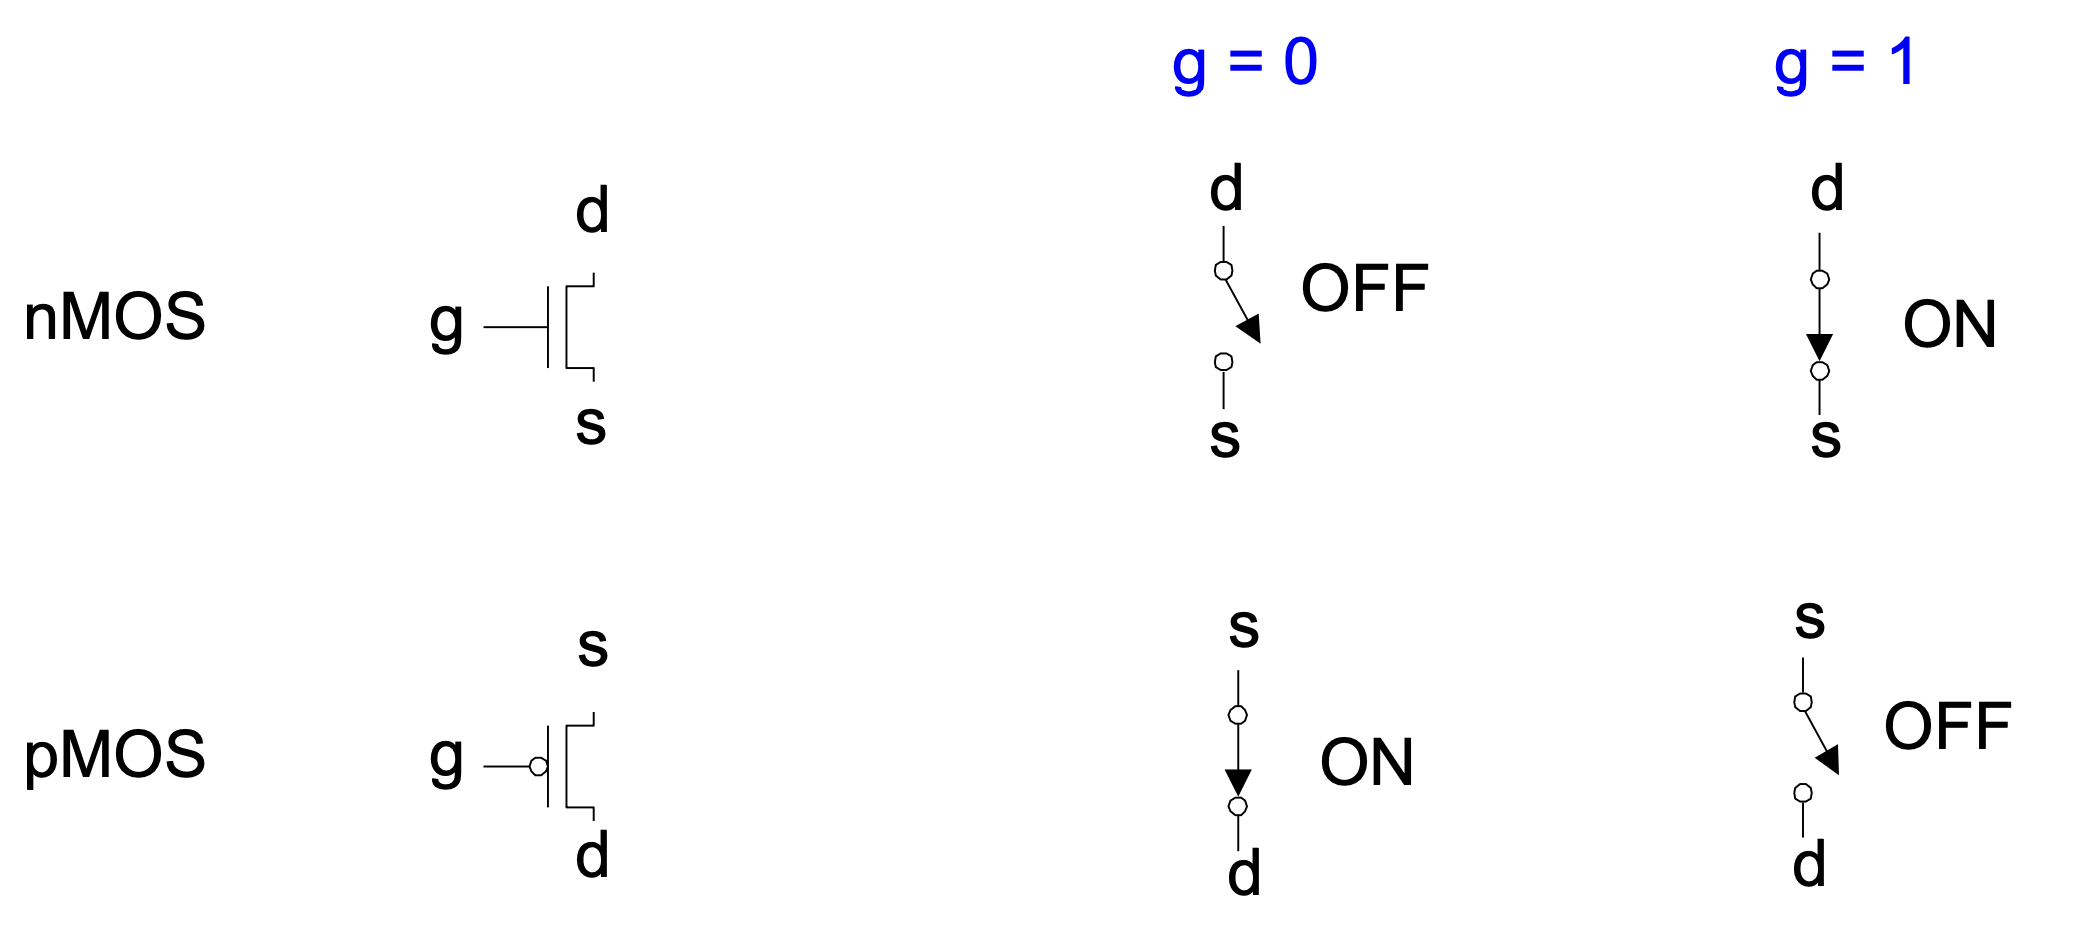
\includegraphics[width=0.8\textwidth]{images/transistor.png}
    \caption{nMOS e pMOS}
\end{figure}

I transistor vengono utilizzati all'interno delle porte logiche per definirne il funzionamento,
di seguito è riportato un esempio per la porta NAND:
\begin{figure}[h]
    \centering
    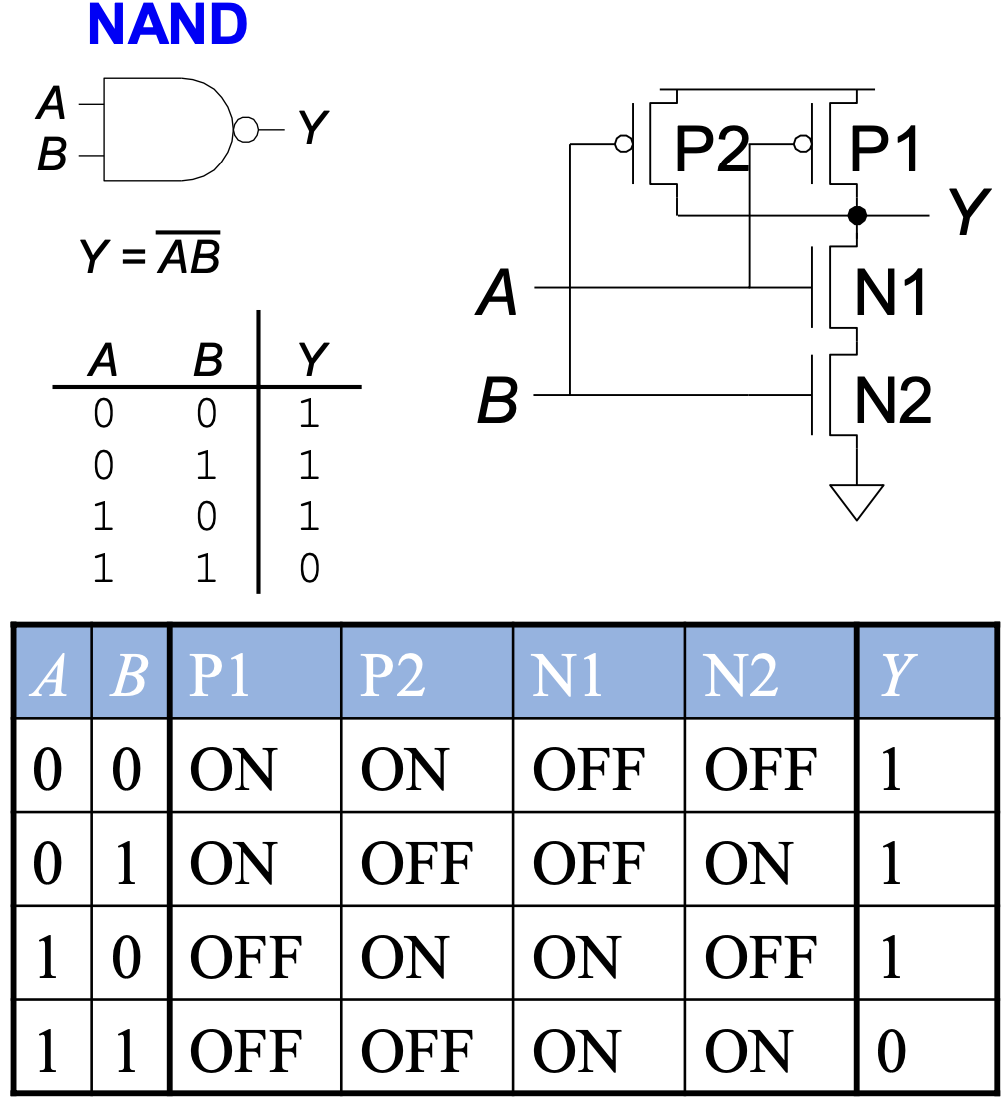
\includegraphics[width=0.6\textwidth]{images/cMOSNAND.png}
    \caption{CMOS NAND Gate}
\end{figure}

Alcune porte logiche non sono strutturalmente definibili in questo modo, ad esempio per la porta AND è necessario
realizzare una porta NAND seguita da una porta NOT.

\end{document}